%% Example presentation
\documentclass[en]{sdqbeamer}

%% Title image
\titleimage{banner_2020_kit}

%% Group logo
%\grouplogo{ISASLogoDE}
\grouplogo{ISASLogoEN}

% Start of the presentation

\title[]{Variational Optimization with Deterministic Sampling for Model Predictive Control}
%\subtitle{according to the design guidelines of 1 August 2020}
\author[Soham Parab, Arion Petrela, Hao Bai]{Soham Parab, Arion Petrela, Hao Bai}
\supervisor{Markus Walker, Xiaozhu Luo}

\date[13\,Nov\,2026]{13 November 2026}

% Literature

\usepackage[citestyle=authoryear,bibstyle=numeric,hyperref,backend=biber]{biblatex}
\addbibresource{presentation.bib}
\bibhang1em

\begin{document}

%Title page
\KITtitleframe

%Table of contents
\begin{frame}{Table of Contents}
\tableofcontents
\end{frame}

\section{Introduction}
\subsection{Motivation: Model predictive control}
\subsection{Variational optimization}
\subsection{Deterministic sampling}
\subsection{Problem Statement}

\section{Methodology}
\subsection{Task definition}
\subsection{System Overview}
\subsection{Optimization methods}
\subsection{Evaluation setup}



\section{Goals}
\subsection{Deliverables}
\subsection{Evaluation criteria}


\section{Project Plan}
\subsection{Timeline (Gantt chart)}

\begin{frame}{Motivation: Model Predictive Control}
	\begin{itemize}
		\item Predict $\rightarrow$ Optimize $\rightarrow$ Apply first input $\rightarrow$ Repeat
		\item Handles nonlinear dynamics and constraints
	\end{itemize}
	\begin{center}
		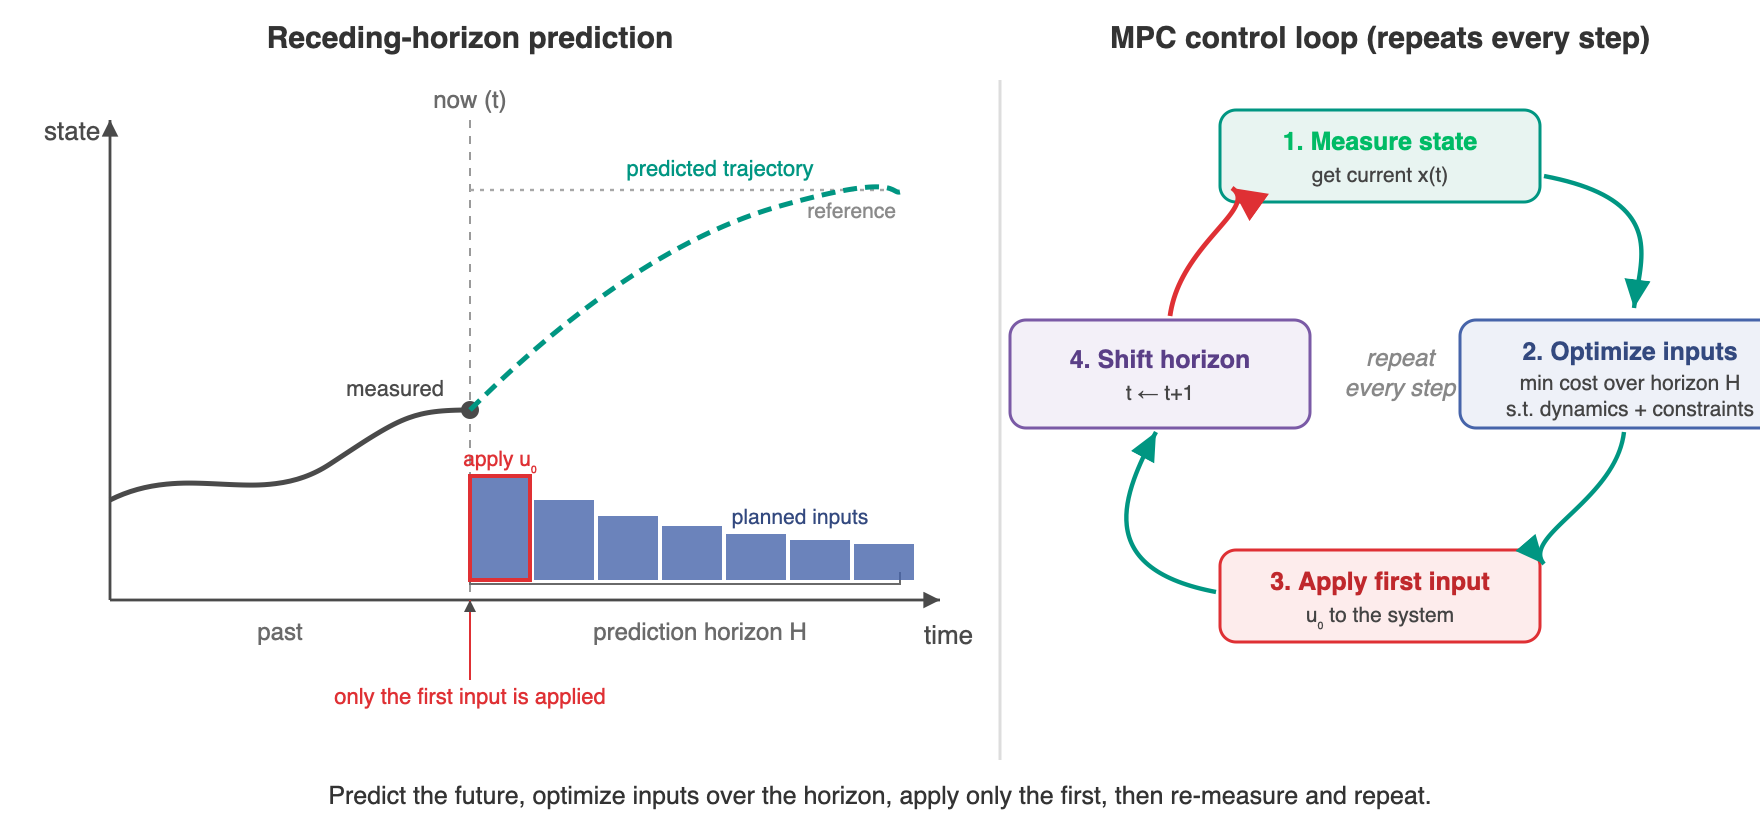
\includegraphics[height=0.62\textheight]{mpc_loop}
	\end{center}
\end{frame}

\begin{frame}{Motivation: Model Predictive Control}
	\begin{itemize}
		\item At each step: find the input sequence $U = (u_0, \ldots, u_{H-1})$ that minimizes the predicted cost $J(U)$
		\item Why it's hard:
		\begin{itemize}
			\item Non-convex $\rightarrow$ prone to local minima
			\item High-dimensional $\rightarrow$ scales with horizon $\times$ inputs
			\item Time-critical $\rightarrow$ re-solved at every control step
		\end{itemize}
	\end{itemize}
	\begin{center}
		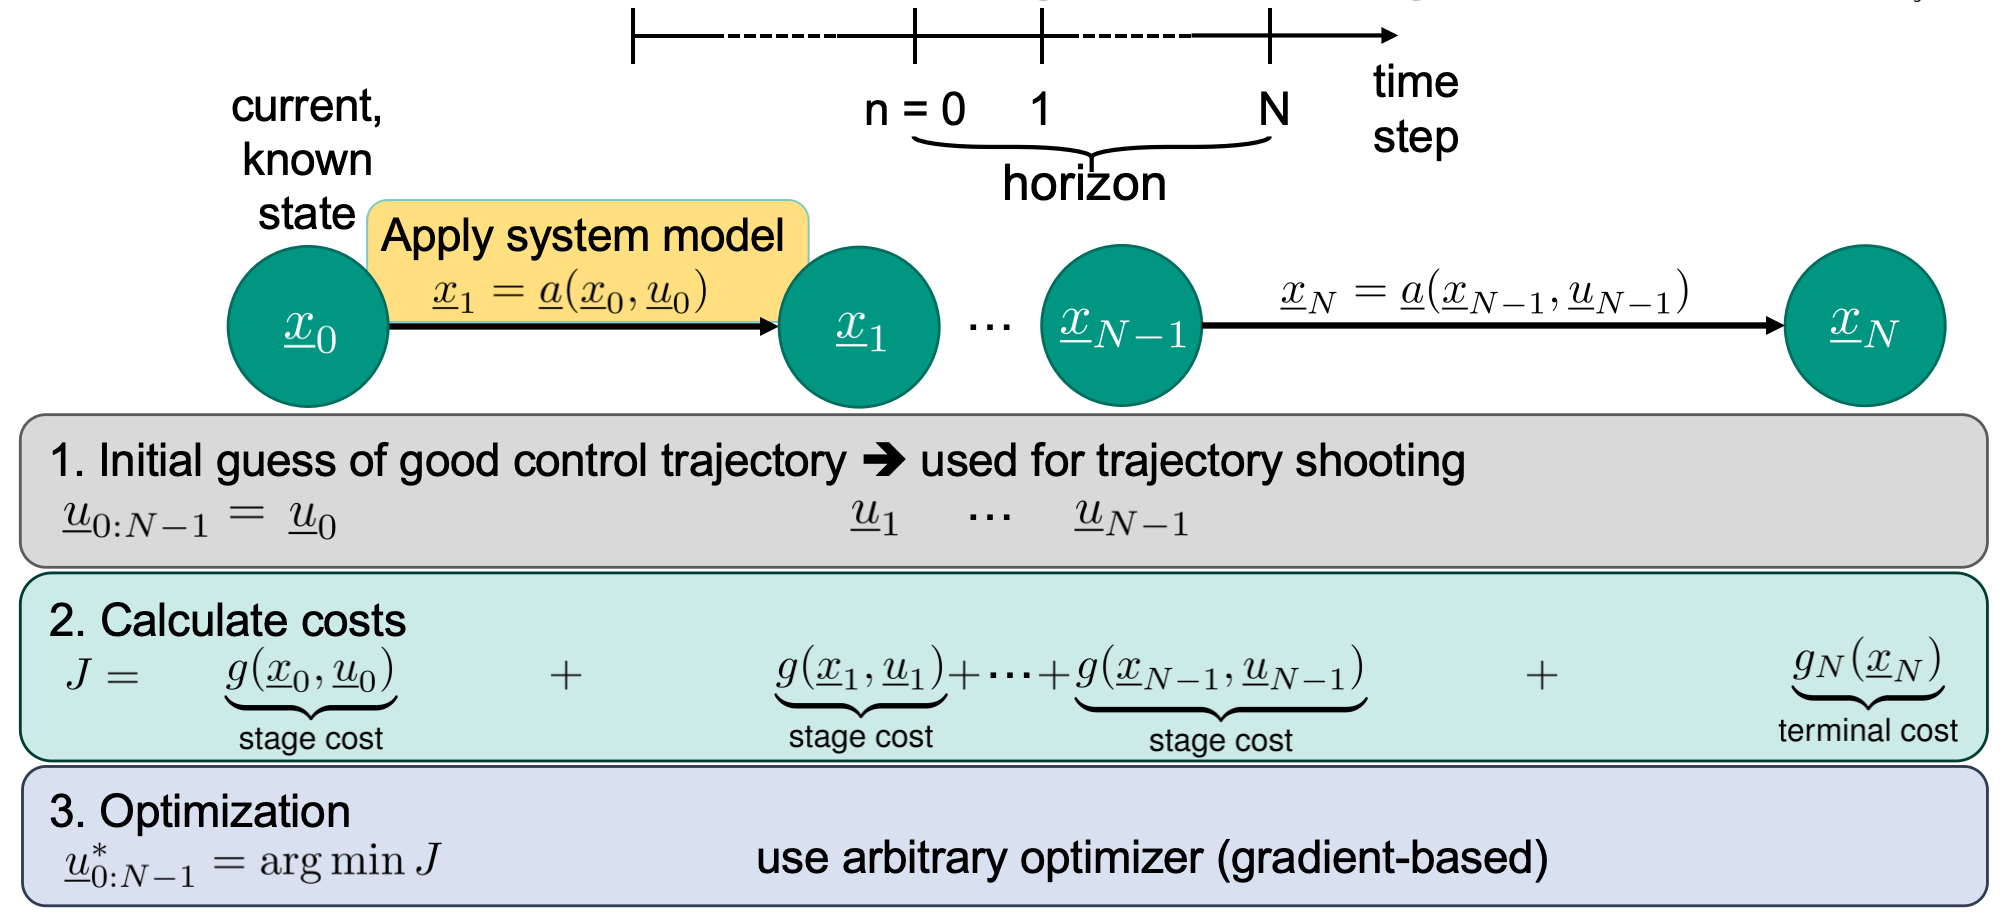
\includegraphics[height=0.5\textheight]{mpc}
	\end{center}
\end{frame}

\begin{frame}{Blocks}
	\begin{contentblock}{Contentblock}
		Colourless block with bold heading.
	\end{contentblock}
	\begin{columns}
		\column{.3\textwidth}
		\begin{greenblock}{Greenblock}
			Default (\texttt{block})
        \end{greenblock}
		\column{.3\textwidth}
		\begin{blueblock}{Blueblock}
			= \texttt{exampleblock}
        \end{blueblock}
		\column{.3\textwidth}
		\begin{redblock}{Redblock}
			= \texttt{alertblock}
        \end{redblock}
	\end{columns}
	\begin{columns}
		\column{.3\textwidth}
        \begin{brownblock}{Brownblock}
        \end{brownblock}
		\column{.3\textwidth}
        \begin{purpleblock}{Purpleblock}
        \end{purpleblock}
		\column{.3\textwidth}
        \begin{cyanblock}{Cyanblock}
        \end{cyanblock}
	\end{columns}
	\begin{columns}
		\column{.3\textwidth}
        \begin{yellowblock}{Yellowblock}
        \end{yellowblock}
		\column{.3\textwidth}
        \begin{lightgreenblock}{Lightgreenblock}
        \end{lightgreenblock}
		\column{.3\textwidth}
        \begin{orangeblock}{Orangeblock}
        \end{orangeblock}
	\end{columns}
	\begin{columns}
		\column{.3\textwidth}
        \begin{grayblock}{Grayblock}
        \end{grayblock}
		\column{.3\textwidth}
		\column{.3\textwidth}
	\end{columns}
\end{frame}



\begin{frame}
        For frames without a title, the header is not shown, and
    the free space can be used for content.
\end{frame}

\begin{frame}[plain]
    For frames with the option \texttt{[plain]}, neither header nor footer is shown.
\end{frame}

\begin{frame}[t]{Example Content}
    For frames with the option \texttt{[t]}, the content is not vertically centred but starts at the top edge.
\end{frame}


\begin{frame}{Example Content: Literature}
    Citation: \cite{klare2021jss}
\end{frame}

\appendix
\beginbackup

\begin{frame}{Literature}
\begin{exampleblock}{Backup Section}
    Slides inserted after \texttt{\textbackslash beginbackup} do not count towards the total number of slides.
\end{exampleblock}

\printbibliography
\end{frame}

\section{Colours}
%% ----------------------------------------
%% | Test slide with defined colours |
%% ----------------------------------------
\begin{frame}{Colour Palette}
\tiny

% GREEN
	\colorbox{kit-green100}{kit-green100}
	\colorbox{kit-green90}{kit-green90}
	\colorbox{kit-green80}{kit-green80}
	\colorbox{kit-green70}{kit-green70}
	\colorbox{kit-green60}{kit-green60}
	\colorbox{kit-green50}{kit-green50}
	\colorbox{kit-green40}{kit-green40}
	\colorbox{kit-green30}{kit-green30}
	\colorbox{kit-green25}{kit-green25}
	\colorbox{kit-green20}{kit-green20}
	\colorbox{kit-green15}{kit-green15}
	\colorbox{kit-green10}{kit-green10}
	\colorbox{kit-green5}{kit-green5}

% BLUE
	\colorbox{kit-blue100}{kit-blue100}
	\colorbox{kit-blue90}{kit-blue90}
	\colorbox{kit-blue80}{kit-blue80}
	\colorbox{kit-blue70}{kit-blue70}
	\colorbox{kit-blue60}{kit-blue60}
	\colorbox{kit-blue50}{kit-blue50}
	\colorbox{kit-blue40}{kit-blue40}
	\colorbox{kit-blue30}{kit-blue30}
	\colorbox{kit-blue25}{kit-blue25}
	\colorbox{kit-blue20}{kit-blue20}
	\colorbox{kit-blue15}{kit-blue15}
	\colorbox{kit-blue10}{kit-blue10}
	\colorbox{kit-blue5}{kit-blue5}

% RED
	\colorbox{kit-red100}{kit-red100}
	\colorbox{kit-red90}{kit-red90}
	\colorbox{kit-red80}{kit-red80}
	\colorbox{kit-red70}{kit-red70}
	\colorbox{kit-red60}{kit-red60}
	\colorbox{kit-red50}{kit-red50}
	\colorbox{kit-red40}{kit-red40}
	\colorbox{kit-red30}{kit-red30}
	\colorbox{kit-red25}{kit-red25}
	\colorbox{kit-red20}{kit-red20}
	\colorbox{kit-red15}{kit-red15}
	\colorbox{kit-red10}{kit-red10}
	\colorbox{kit-red5}{kit-red5}

% GREY
	\colorbox{kit-gray100}{\color{white}kit-gray100}
	\colorbox{kit-gray90}{\color{white}kit-gray90}
	\colorbox{kit-gray80}{\color{white}kit-gray80}
	\colorbox{kit-gray70}{\color{white}kit-gray70}
	\colorbox{kit-gray60}{\color{white}kit-gray60}
	\colorbox{kit-gray50}{\color{white}kit-gray50}
	\colorbox{kit-gray40}{kit-gray40}
	\colorbox{kit-gray30}{kit-gray30}
	\colorbox{kit-gray25}{kit-gray25}
	\colorbox{kit-gray20}{kit-gray20}
	\colorbox{kit-gray15}{kit-gray15}
	\colorbox{kit-gray10}{kit-gray10}
	\colorbox{kit-gray5}{kit-gray5}

% Orange
	\colorbox{kit-orange100}{kit-orange100}
	\colorbox{kit-orange90}{kit-orange90}
	\colorbox{kit-orange80}{kit-orange80}
	\colorbox{kit-orange70}{kit-orange70}
	\colorbox{kit-orange60}{kit-orange60}
	\colorbox{kit-orange50}{kit-orange50}
	\colorbox{kit-orange40}{kit-orange40}
	\colorbox{kit-orange30}{kit-orange30}
	\colorbox{kit-orange25}{kit-orange25}
	\colorbox{kit-orange20}{kit-orange20}
	\colorbox{kit-orange15}{kit-orange15}
	\colorbox{kit-orange10}{kit-orange10}
	\colorbox{kit-orange5}{kit-orange5}

% lightgreen
	\colorbox{kit-lightgreen100}{kit-lightgreen100}
	\colorbox{kit-lightgreen90}{kit-lightgreen90}
	\colorbox{kit-lightgreen80}{kit-lightgreen80}
	\colorbox{kit-lightgreen70}{kit-lightgreen70}
	\colorbox{kit-lightgreen60}{kit-lightgreen60}
	\colorbox{kit-lightgreen50}{kit-lightgreen50}
	\colorbox{kit-lightgreen40}{kit-lightgreen40}
	\colorbox{kit-lightgreen30}{kit-lightgreen30}
	\colorbox{kit-lightgreen25}{kit-lightgreen25}
	\colorbox{kit-lightgreen20}{kit-lightgreen20}
	\colorbox{kit-lightgreen15}{kit-lightgreen15}
	\colorbox{kit-lightgreen10}{kit-lightgreen10}
	\colorbox{kit-lightgreen5}{kit-lightgreen5}

% Brown
	\colorbox{kit-brown100}{kit-brown100}
	\colorbox{kit-brown90}{kit-brown90}
	\colorbox{kit-brown80}{kit-brown80}
	\colorbox{kit-brown70}{kit-brown70}
	\colorbox{kit-brown60}{kit-brown60}
	\colorbox{kit-brown50}{kit-brown50}
	\colorbox{kit-brown40}{kit-brown40}
	\colorbox{kit-brown30}{kit-brown30}
	\colorbox{kit-brown25}{kit-brown25}
	\colorbox{kit-brown20}{kit-brown20}
	\colorbox{kit-brown15}{kit-brown15}
	\colorbox{kit-brown10}{kit-brown10}
	\colorbox{kit-brown5}{kit-brown5}

% Purple
	\colorbox{kit-purple100}{kit-purple100}
	\colorbox{kit-purple90}{kit-purple90}
	\colorbox{kit-purple80}{kit-purple80}
	\colorbox{kit-purple70}{kit-purple70}
	\colorbox{kit-purple60}{kit-purple60}
	\colorbox{kit-purple50}{kit-purple50}
	\colorbox{kit-purple40}{kit-purple40}
	\colorbox{kit-purple30}{kit-purple30}
	\colorbox{kit-purple25}{kit-purple25}
	\colorbox{kit-purple20}{kit-purple20}
	\colorbox{kit-purple15}{kit-purple15}
	\colorbox{kit-purple10}{kit-purple10}
	\colorbox{kit-purple5}{kit-purple5}

% Cyan
	\colorbox{kit-cyan100}{kit-cyan100}
	\colorbox{kit-cyan90}{kit-cyan90}
	\colorbox{kit-cyan80}{kit-cyan80}
	\colorbox{kit-cyan70}{kit-cyan70}
	\colorbox{kit-cyan60}{kit-cyan60}
	\colorbox{kit-cyan50}{kit-cyan50}
	\colorbox{kit-cyan40}{kit-cyan40}
	\colorbox{kit-cyan30}{kit-cyan30}
	\colorbox{kit-cyan25}{kit-cyan25}
	\colorbox{kit-cyan20}{kit-cyan20}
	\colorbox{kit-cyan15}{kit-cyan15}
	\colorbox{kit-cyan10}{kit-cyan10}
	\colorbox{kit-cyan5}{kit-cyan5}

\end{frame}
%% ----------------------------------------
%% | /Test slide with defined colours |
%% ----------------------------------------
\backupend

\end{document}